\begin{frame}{Anforderung}
	\begin{itemize}
		\item Implementierung der Form für Einen neuen Agenten
		\item Ein Lauffähiges Modell für die Simulation eines Pferdes
	\end{itemize}
\end{frame}

\begin{frame}{Meine Aufgaben}
	\begin{itemize}
		\item Einarbeiten in VadereState
		\item Einarbeiten in VadereUtils
		\item Einführung einer neuen Form VEllipse
		\item Bugfix "Nur ein Horse Modell wird im Simulator gezeichnet"
	\end{itemize}
\end{frame}

\begin{frame}{Topography}
	\begin{figure}
		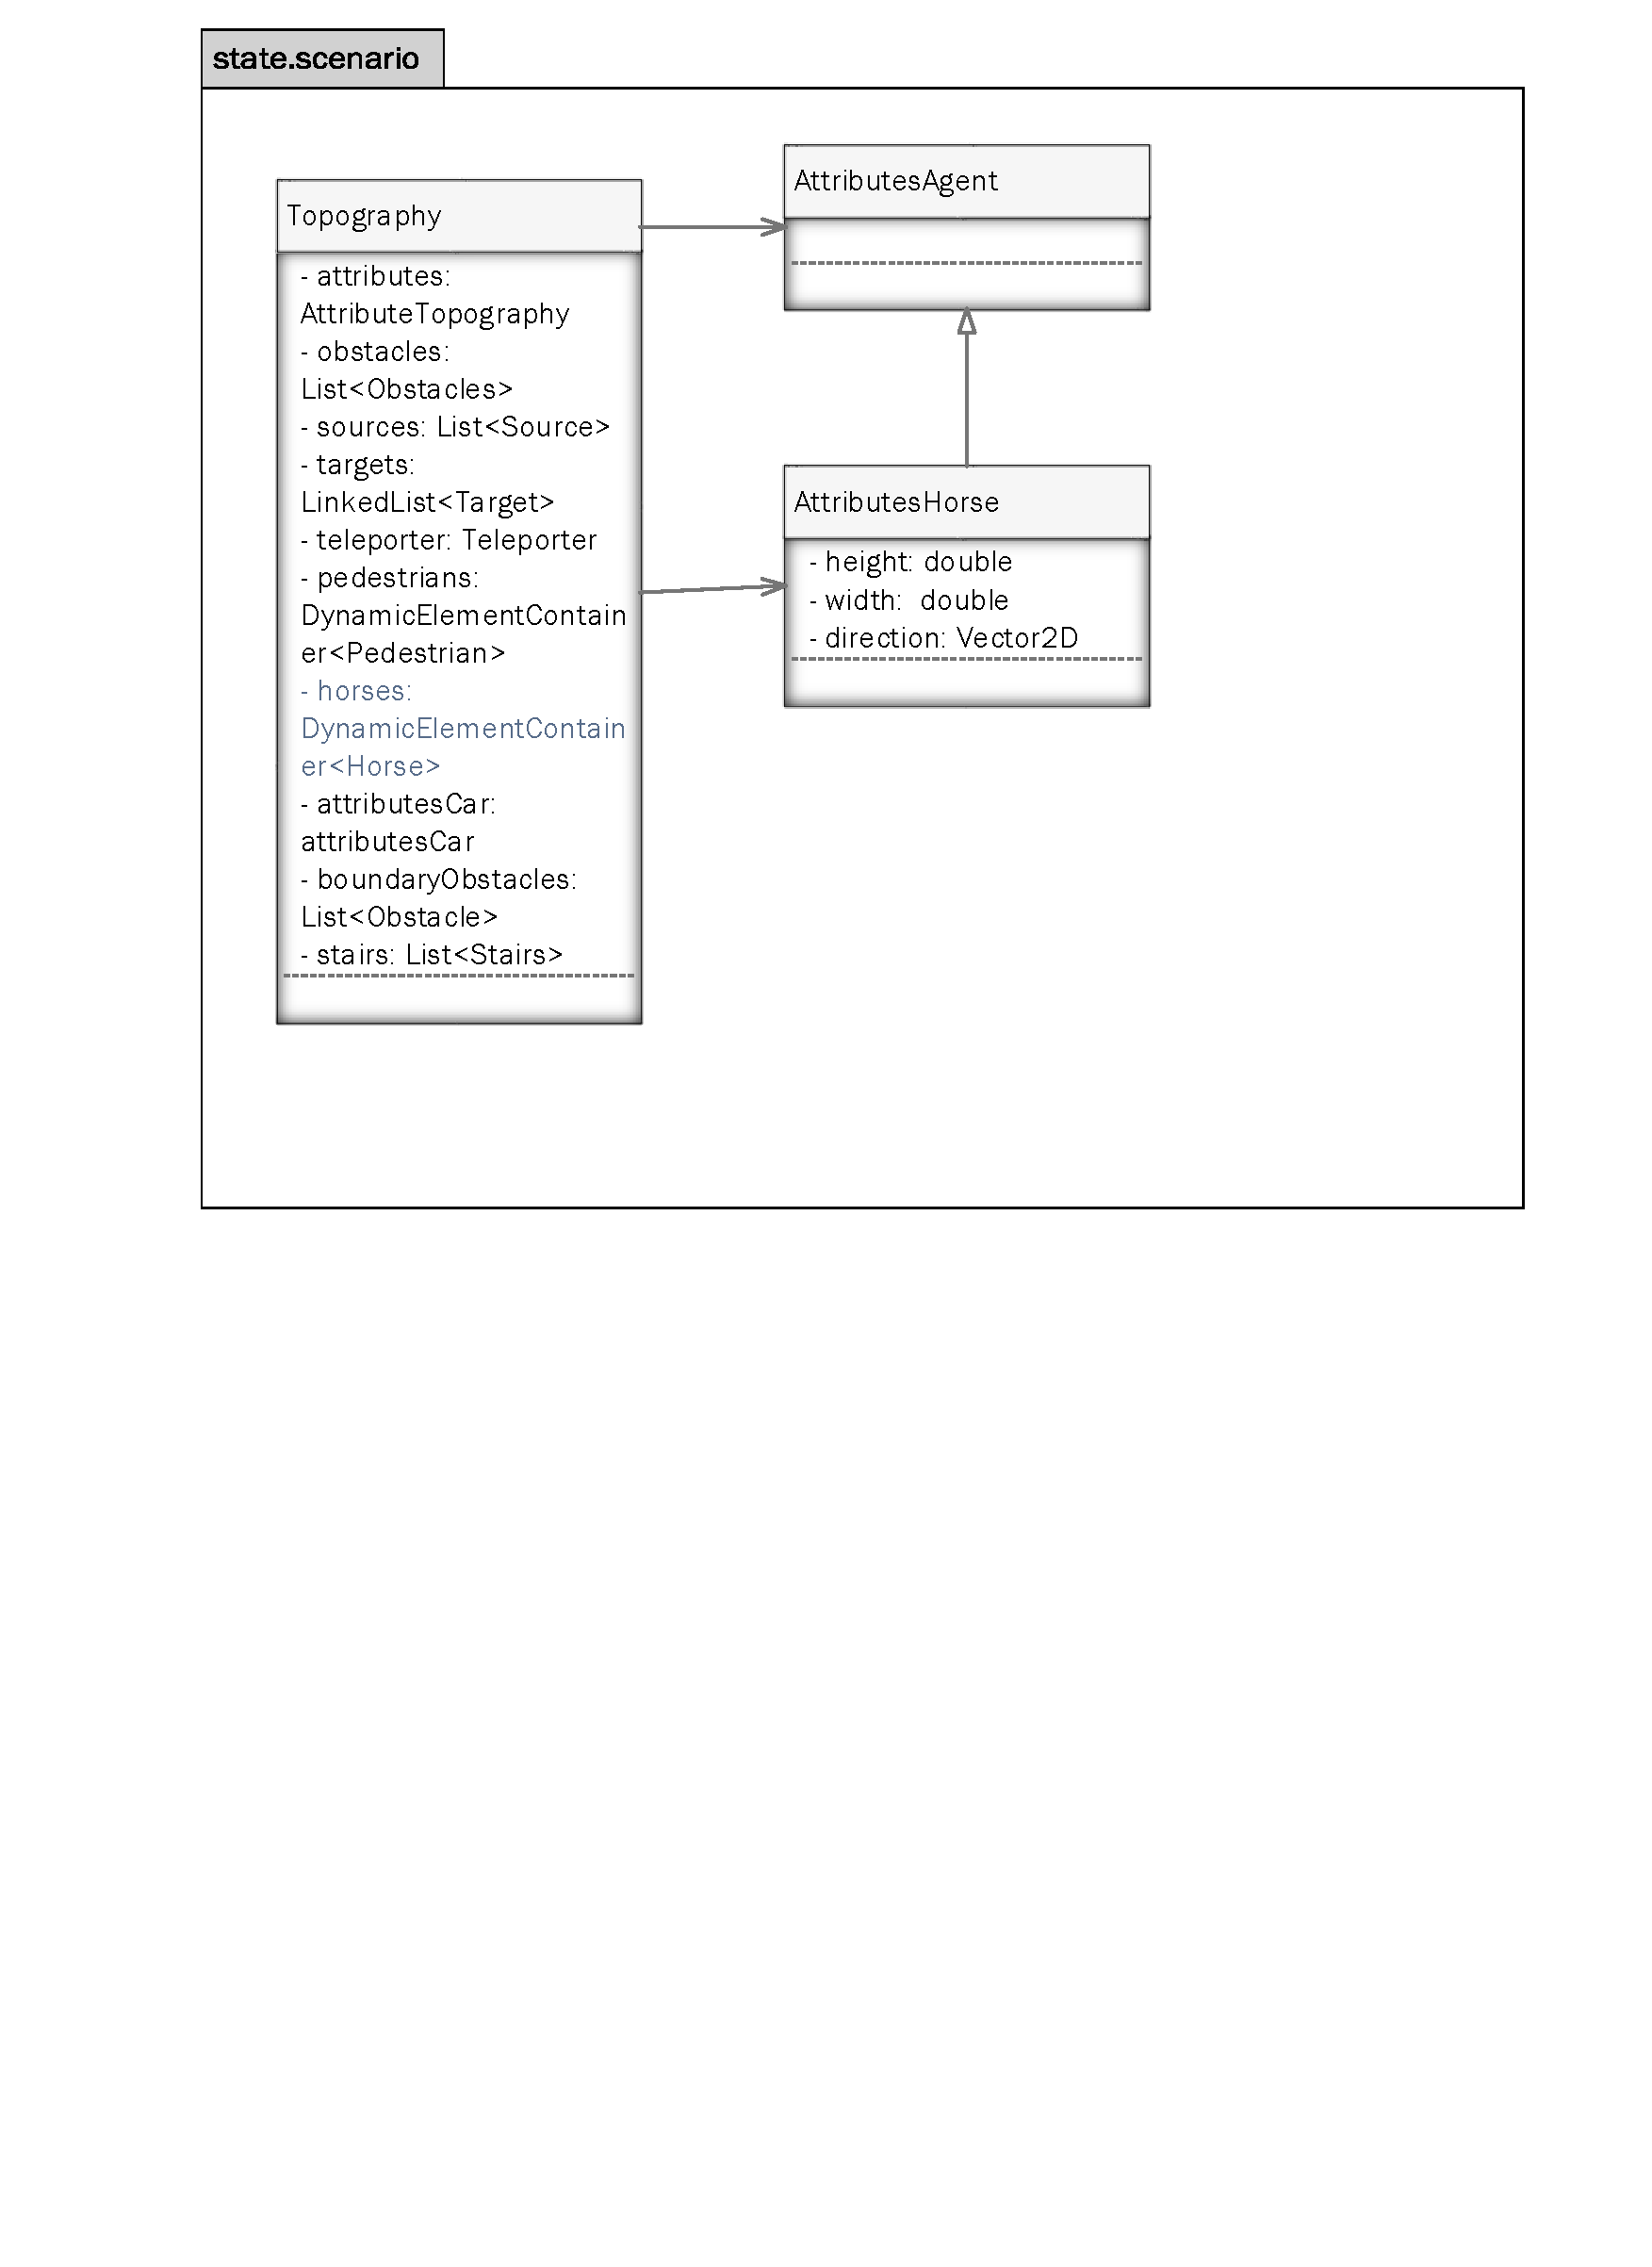
\includegraphics[width=\textwidth, keepaspectratio]{appendix/uml/Topography.pdf}
	\end{figure}
\end{frame}

\begin{frame}{Ellipse}
	\begin{figure}
		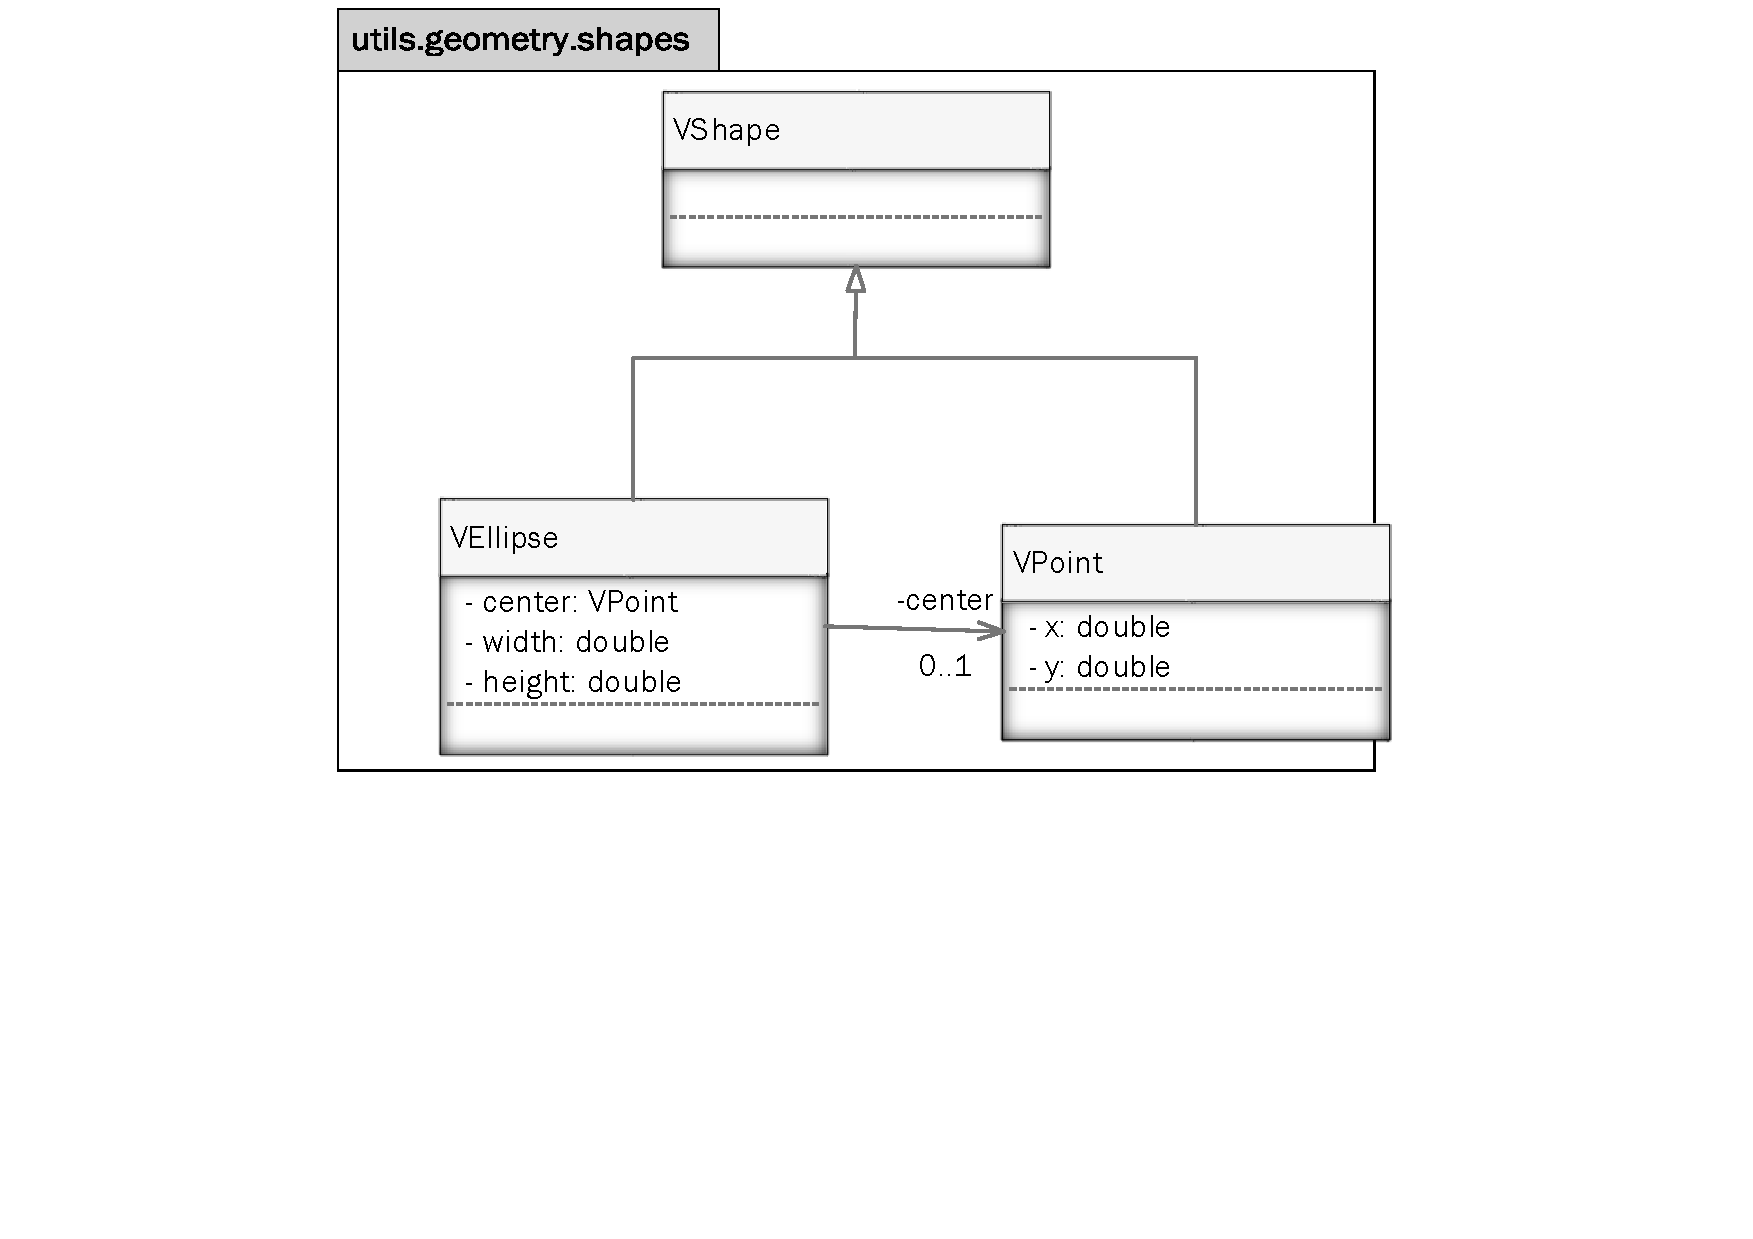
\includegraphics[width=\textwidth, keepaspectratio]{appendix/uml/Ellipse.pdf}
	\end{figure}
\end{frame}

\begin{frame}{Fazit}
	\begin{itemize}
		\item Das Pferd benutzt die Form Ellipse 
		\item Mehrere Pferde können das Ziel erreichen
		\item Serialisierung der neuen Form
	\end{itemize}
\end{frame}

\begin{frame}{Retrospektive}
	\begin{itemize}
		\item{Fand ich gut:}
		\begin{itemize}
			\item{Erreichbarkeit des Teams}
			\item{Arbeiten mit neuen Tools}
			\item{Hilfebereitschaft des Teams}
		\end{itemize}
		\item{Könnte besser sein:}
		\begin{itemize}
			\item{Pünktlichkeit}
			\item{Kürzere Dailies}
		\end{itemize}
		\item{Mein Anteil: 23\%}
	\end{itemize}
\end{frame}